\documentclass[titlepage]{article}
\usepackage[english]{babel}
\usepackage[utf8]{inputenc}
\usepackage{fancyhdr}
\usepackage{amsfonts} 
\usepackage{amsmath}
\usepackage{glossaries}
\usepackage[colorlinks]{hyperref}
\usepackage{venndiagram}
\usepackage{tikz}

\pagestyle{fancy}
\fancyhf{}
\rhead{Joshua Murphy}
\lhead{Course Notes - COMP 1002}
\rfoot{Page \thepage}
\title{COMP 1002 Survival Guide}
\author{Joshua Murphy}
\date{\today}
\newglossaryentry{implication}{%
  name={implication},%
  description={valid knowledge used to refer to an area of human endeavour, an autonomous computer activity, or other specialized discipline}}

\newglossaryentry{set}{%
  name={set},%
  description={A collection of objects}}


\makeglossaries
\begin{document}
\maketitle
\tableofcontents{}
\pagebreak


% Begin section on propositional logic 
\section{Propositional Logic}


\subsection{Implication}
In logic, an \gls{implication} is a 


\begin{equation}p \to q \end{equation}
This is read as ``\textit{p implies q.}'' In this case $P$ = it is raining, 
and $Q$ = there are clouds. 
Insert truth table
\subsubsection{Example:}
$p \to q$
\subsection{Biconditional}
\begin{equation}
p \iff q \end{equation}
This is read as ``\textit{p if and only if q.}'' Both $P$ and $Q$ must be the
same value. This differs from $\wedge$ in which both values must be
\textit{true.} For example, $P$ = taking a flight and $Q$ = buying a ticket. It
is false when they have opposite values. You can take the flight if and only if
you buy a ticket.

$\equiv \in \notin \emptyset \forall \exists \rightarrow \leftrightarrow \sigma
\psi \phi $



% Begin section of Predicates, quantifiers and sets.
\section{Predicates, Quantifiers, Sets}
\subsection{Sets}

A \gls{set} is a collection of objects: \\
\newline $ \emptyset $ for the empty set \\
$ \mathbb{S} = \{1, 2, 3\}$ \\ 
$ \mathbb{N} = \{ 1,3,3\cdots\}$  is the set of \textit{natural} numbers. \\
$ \mathbb{Z} = \{\cdots, -2, -1, 0, 1, 2 \cdots\} $ is the set of integers \\
\newline So, on forth  for real numbers, complex, rational, etc.

\subsubsection{Set Elements}

Means that element $a$ is in set S: 
\begin{equation}
 a \in S 
\end{equation}
Means $a$ is not in S:
\begin{equation}
 a \notin S
\end{equation}
\newline Susan is not a bankteller, i.e  Susan $\notin$ Banktellers: \newline
\newline 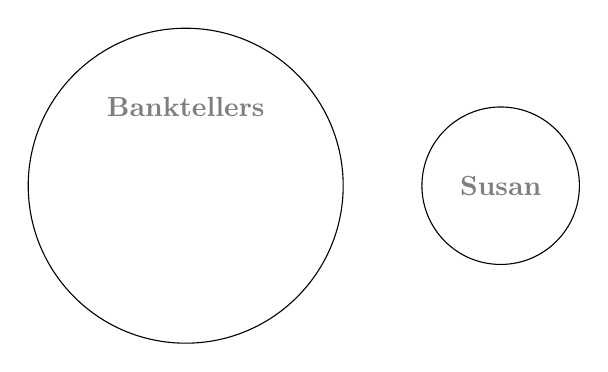
\begin{tikzpicture} 
    \begin{scope}[shift={(0cm,-2cm)}, fill opacity=0.5]
        \draw[fill=white, draw = black] (-1.5,0) circle (2);
        \draw[fill=white, draw = black] (2.5,0) circle (1);
    \node at (-1.5,1) (A) {\textbf{Banktellers}};
    \node at (2.5,0) (B) {\textbf{Susan}};
    \end{scope}
\end{tikzpicture} \\
\newline Susan is a bankteller, i.e Susan $\in$ Banktellers: \newline
\newline 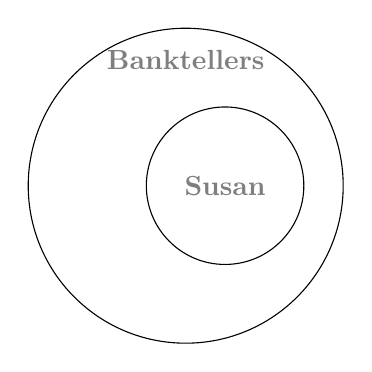
\begin{tikzpicture}
    \begin{scope}[shift={(0cm,-2cm)}, fill opacity=0.5]
        \draw[fill=white, draw = black] (-1.5,0) circle (2);
        \draw[fill=white, draw = black] (-1,0) circle (1);
    \node at (-1.5,1.6) (A) {\textbf{Banktellers}};
    \node at (-1,0) (B) {\textbf{Susan}};
    \end{scope}
\end{tikzpicture} \\


% \begin{venndiagram2sets}[
%        labelOnlyA={Susan},
%        labelOnlyB={2},]
%\end{venndiagram2sets}


% Import rest of sections here . . . 
% \include{cool}

\printglossaries
\end{document}
